\subsection{From physics to computation}
To be able to do reservoir simulation, we start with a physicist who model fluid flow inside porous medium.
%
From this model, we can obtain some physical equations.
%
Then we discretize the reservoir into cells and we use a finite difference schema.
%
For each cell of the reservoir, we can compute a non-linear equation of each variables (e.g.: pressure, oil saturation)
%
To solve the non-linear systems of equation, we use the Newton–Raphson method.
%
This method is iterative, we begins with an initial guess $X_0$ reasonably close to the solution $X_n$ which satisfied $F(X_n) = 0$.

%   (-_-)   %
\begin{figure}[!ht]
  \centering
  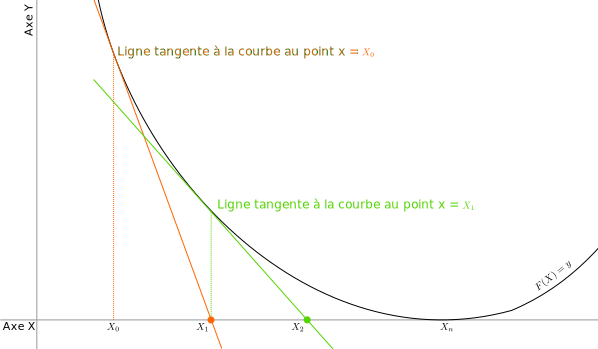
\includegraphics[width=\textwidth]{newton}
  \caption{Example of two Newton steps in one dimension space.
    Each tangent lines correspond to a linear equation to solve.}
\label{newton}
\end{figure}

The example in the figure~\ref{newton} is only in one dimension but it's quite the same approach that can be done when we work with an arbitrary number of dimensions.
%
Linear equations of reservoir siluation can be represent as large sparse matrices.
%
Each row represent all interactions between an element and its direct neighbors.
%
So in a regular mesh, there can have up to seven small dense block per row.
%
Sparse linear algebra solvers, like GMRES, are then utilize to solve all linear problems use in the Newton method.
%
Let's focus on linear algebra.
